\chapter{Programming concept}

 The main language for the implementation of the functionality of the
 dynamic runtime environment functionality is Perl. And it is solely required (exceptions are the
 integration with the Grid Manager and the Web server) for the Janitor. In
 the pre-web-service implementation the Catalog remains a static web page.
 The Perl code is split into multiple modules as depicted in Figure~\ref{fig:janitorDependencies}. 
 The modules can be separated into two
 functional groups. One addresses the retrieval of information from
 the Catalog's RDF file in the left major branch of the figure. The other
 addresses the process of fetching and installing the packages.

 \begin{landscape}
\begin{figure}[!h]
\vspace{4cm}
 \begin{center} 
%    \resizebox{24cm}{!}{
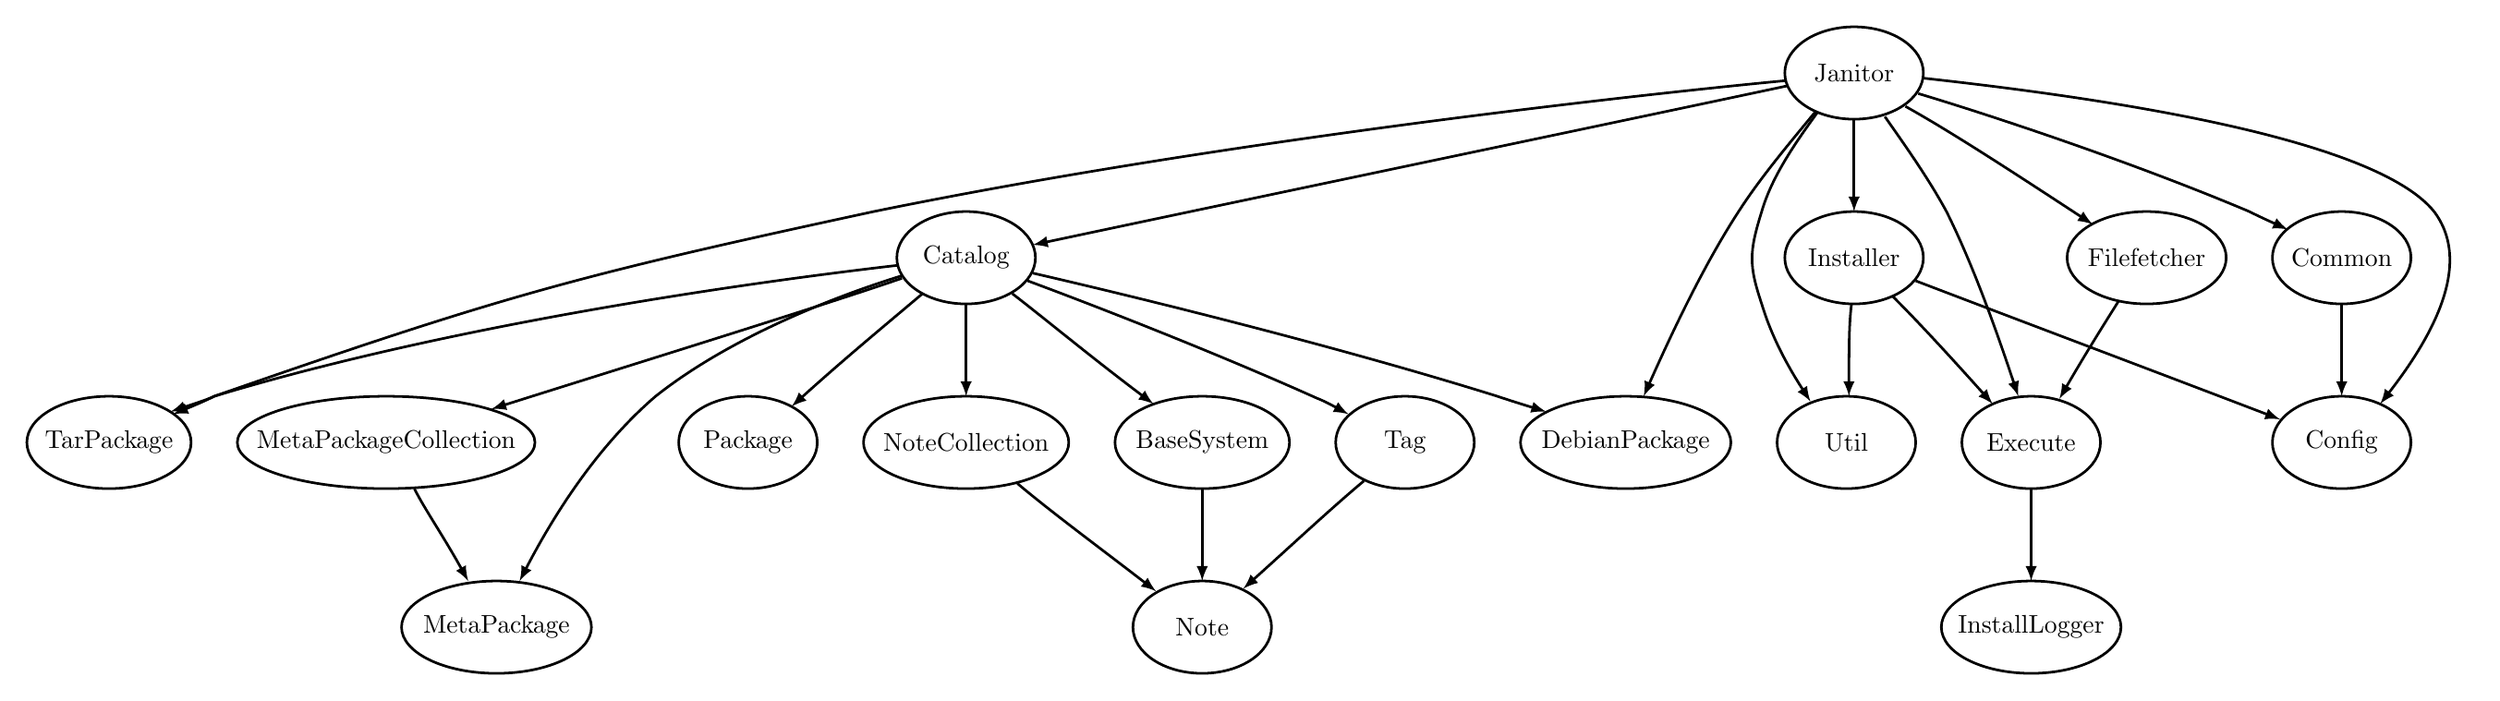
\begin{tikzpicture}[>=latex,line join=bevel,]
  \pgfsetlinewidth{1bp}
%%
\pgfsetcolor{black}
  % Edge: Installer -> Util
  \draw [->] (711bp,144bp) .. controls (710bp,136bp) and (710bp,127bp)  .. (710bp,108bp);
  % Edge: Janitor -> Filefetcher
  \draw [->] (732bp,221bp) .. controls (750bp,211bp) and (776bp,194bp)  .. (805bp,175bp);
  % Edge: Catalog -> Tag
  \draw [->] (390bp,153bp) .. controls (417bp,143bp) and (463bp,125bp)  .. (501bp,108bp) .. controls (503bp,107bp) and (504bp,107bp)  .. (515bp,101bp);
  % Edge: BaseSystem -> Note
  \draw [->] (458bp,72bp) .. controls (458bp,64bp) and (458bp,55bp)  .. (458bp,36bp);
  % Edge: Installer -> Execute
  \draw [->] (727bp,147bp) .. controls (737bp,137bp) and (749bp,124bp)  .. (766bp,105bp);
  % Edge: Janitor -> Catalog
  \draw [->] (686bp,229bp) .. controls (625bp,216bp) and (472bp,184bp)  .. (392bp,167bp);
  % Edge: Catalog -> MetaPackage
  \draw [->] (341bp,155bp) .. controls (315bp,147bp) and (274bp,131bp)  .. (245bp,108bp) .. controls (224bp,90bp) and (207bp,65bp)  .. (192bp,36bp);
  % Edge: Janitor -> TarPackage
  \draw [->] (685bp,231bp) .. controls (622bp,225bp) and (462bp,207bp)  .. (330bp,180bp) .. controls (214bp,155bp) and (185bp,147bp)  .. (73bp,108bp) .. controls (71bp,107bp) and (69bp,106bp)  .. (57bp,101bp);
  % Edge: Filefetcher -> Execute
  \draw [->] (815bp,145bp) .. controls (810bp,137bp) and (803bp,126bp)  .. (792bp,107bp);
  % Edge: Janitor -> Config
  \draw [->] (739bp,232bp) .. controls (793bp,226bp) and (913bp,211bp)  .. (938bp,180bp) .. controls (953bp,160bp) and (938bp,132bp)  .. (917bp,105bp);
  % Edge: Janitor -> Execute
  \draw [->] (724bp,217bp) .. controls (731bp,207bp) and (741bp,193bp)  .. (748bp,180bp) .. controls (758bp,160bp) and (767bp,135bp)  .. (776bp,108bp);
  % Edge: Catalog -> TarPackage
  \draw [->] (339bp,159bp) .. controls (287bp,153bp) and (169bp,137bp)  .. (73bp,108bp) .. controls (71bp,107bp) and (68bp,106bp)  .. (56bp,102bp);
  % Edge: Catalog -> DebianPackage
  \draw [->] (392bp,156bp) .. controls (431bp,147bp) and (509bp,128bp)  .. (573bp,108bp) .. controls (576bp,107bp) and (579bp,106bp)  .. (592bp,102bp);
  % Edge: Installer -> Config
  \draw [->] (736bp,153bp) .. controls (770bp,140bp) and (831bp,117bp)  .. (878bp,99bp);
  % Edge: Tag -> Note
  \draw [->] (521bp,75bp) .. controls (509bp,65bp) and (494bp,51bp)  .. (474bp,33bp);
  % Edge: MetaPackageCollection -> MetaPackage
  \draw [->] (151bp,72bp) .. controls (155bp,64bp) and (162bp,54bp)  .. (172bp,36bp);
  % Edge: Common -> Config
  \draw [->] (902bp,144bp) .. controls (902bp,136bp) and (902bp,127bp)  .. (902bp,108bp);
  % Edge: Janitor -> DebianPackage
  \draw [->] (697bp,219bp) .. controls (688bp,208bp) and (676bp,194bp)  .. (667bp,180bp) .. controls (654bp,160bp) and (642bp,135bp)  .. (630bp,108bp);
  % Edge: Catalog -> Package
  \draw [->] (349bp,148bp) .. controls (336bp,137bp) and (319bp,123bp)  .. (298bp,104bp);
  % Edge: Catalog -> NoteCollection
  \draw [->] (366bp,144bp) .. controls (366bp,136bp) and (366bp,127bp)  .. (366bp,108bp);
  % Edge: Janitor -> Installer
  \draw [->] (712bp,216bp) .. controls (712bp,208bp) and (712bp,199bp)  .. (712bp,180bp);
  % Edge: Janitor -> Util
  \draw [->] (698bp,219bp) .. controls (690bp,208bp) and (680bp,194bp)  .. (676bp,180bp) .. controls (671bp,164bp) and (671bp,159bp)  .. (676bp,144bp) .. controls (679bp,134bp) and (684bp,123bp)  .. (695bp,106bp);
  % Edge: Execute -> InstallLogger
  \draw [->] (781bp,72bp) .. controls (781bp,64bp) and (781bp,55bp)  .. (781bp,36bp);
  % Edge: Janitor -> Common
  \draw [->] (737bp,226bp) .. controls (767bp,217bp) and (821bp,199bp)  .. (866bp,180bp) .. controls (868bp,179bp) and (870bp,178bp)  .. (881bp,173bp);
  % Edge: NoteCollection -> Note
  \draw [->] (386bp,74bp) .. controls (399bp,63bp) and (418bp,49bp)  .. (440bp,32bp);
  % Edge: Catalog -> BaseSystem
  \draw [->] (384bp,148bp) .. controls (397bp,138bp) and (415bp,123bp)  .. (439bp,105bp);
  % Edge: Catalog -> MetaPackageCollection
  \draw [->] (341bp,154bp) .. controls (306bp,142bp) and (238bp,121bp)  .. (181bp,103bp);
  % Node: Note
\begin{scope}
  \pgfsetstrokecolor{black}
  \draw (458bp,18bp) ellipse (27bp and 18bp);
  \draw (458bp,18bp) node {Note};
\end{scope}
  % Node: Execute
\begin{scope}
  \pgfsetstrokecolor{black}
  \draw (781bp,90bp) ellipse (27bp and 18bp);
  \draw (781bp,90bp) node {Execute};
\end{scope}
  % Node: Package
\begin{scope}
  \pgfsetstrokecolor{black}
  \draw (281bp,90bp) ellipse (27bp and 18bp);
  \draw (281bp,90bp) node {Package};
\end{scope}
  % Node: DebianPackage
\begin{scope}
  \pgfsetstrokecolor{black}
  \draw (623bp,90bp) ellipse (41bp and 18bp);
  \draw (623bp,90bp) node {DebianPackage};
\end{scope}
  % Node: Config
\begin{scope}
  \pgfsetstrokecolor{black}
  \draw (902bp,90bp) ellipse (27bp and 18bp);
  \draw (902bp,90bp) node {Config};
\end{scope}
  % Node: MetaPackage
\begin{scope}
  \pgfsetstrokecolor{black}
  \draw (183bp,18bp) ellipse (37bp and 18bp);
  \draw (183bp,18bp) node {MetaPackage};
\end{scope}
  % Node: NoteCollection
\begin{scope}
  \pgfsetstrokecolor{black}
  \draw (366bp,90bp) ellipse (40bp and 18bp);
  \draw (366bp,90bp) node {NoteCollection};
\end{scope}
  % Node: Util
\begin{scope}
  \pgfsetstrokecolor{black}
  \draw (709bp,90bp) ellipse (27bp and 18bp);
  \draw (709bp,90bp) node {Util};
\end{scope}
  % Node: Catalog
\begin{scope}
  \pgfsetstrokecolor{black}
  \draw (366bp,162bp) ellipse (27bp and 18bp);
  \draw (366bp,162bp) node {Catalog};
\end{scope}
  % Node: Tag
\begin{scope}
  \pgfsetstrokecolor{black}
  \draw (537bp,90bp) ellipse (27bp and 18bp);
  \draw (537bp,90bp) node {Tag};
\end{scope}
  % Node: Filefetcher
\begin{scope}
  \pgfsetstrokecolor{black}
  \draw (826bp,162bp) ellipse (31bp and 18bp);
  \draw (826bp,162bp) node {Filefetcher};
\end{scope}
  % Node: Common
\begin{scope}
  \pgfsetstrokecolor{black}
  \draw (902bp,162bp) ellipse (27bp and 18bp);
  \draw (902bp,162bp) node {Common};
\end{scope}
  % Node: MetaPackageCollection
\begin{scope}
  \pgfsetstrokecolor{black}
  \draw (140bp,90bp) ellipse (58bp and 18bp);
  \draw (140bp,90bp) node {MetaPackageCollection};
\end{scope}
  % Node: Installer
\begin{scope}
  \pgfsetstrokecolor{black}
  \draw (712bp,162bp) ellipse (27bp and 18bp);
  \draw (712bp,162bp) node {Installer};
\end{scope}
  % Node: Janitor
\begin{scope}
  \pgfsetstrokecolor{black}
  \draw (712bp,234bp) ellipse (27bp and 18bp);
  \draw (712bp,234bp) node {Janitor};
\end{scope}
  % Node: TarPackage
\begin{scope}
  \pgfsetstrokecolor{black}
  \draw (32bp,90bp) ellipse (32bp and 18bp);
  \draw (32bp,90bp) node {TarPackage};
\end{scope}
  % Node: BaseSystem
\begin{scope}
  \pgfsetstrokecolor{black}
  \draw (458bp,90bp) ellipse (34bp and 18bp);
  \draw (458bp,90bp) node {BaseSystem};
\end{scope}
  % Node: InstallLogger
\begin{scope}
  \pgfsetstrokecolor{black}
  \draw (781bp,18bp) ellipse (35bp and 18bp);
  \draw (781bp,18bp) node {InstallLogger};
\end{scope}
%
\end{tikzpicture}

}
    \includegraphics[width=24cm]{images/dependencies.png}
    \mycaption{Modules of the Janitor and their dependencies}{}
 \end{center} 
\vfill
 \label{fig:janitorDependencies} 
\end{figure}
 \end{landscape}

In order to get a more detailed view on the full functionality of the envisioned system it is suggested to consult the 
Design Document\footnote{\href{http://www.knowarc.eu/documents/Knowarc_D1.1-1_07.pdf}
{http://www.knowarc.eu/documents/Knowarc\_D1.1-1\_07.pdf}}.




\section{States of runtime environments}
A major motivation for the managed, manual initiation of dynamic RE
installation is the subsequent manual verification of the installed
packages -- prior to their use in production.
With an automation of the installation, the verification of
that process shall be performed externally to that process.  At this
time, only the automation of the installation has been implemented.
To reflect the progress the external verification has made, REs
are said to be in states. The current implementation lists
installable REs aside the installed REs in the grid information system,
in order to stimulate grid clients to submit packages. The here described
states will be represented to the clients in upcoming developments.

These states are specific for every compute element (CE) and communicated
between the Janitor and the Execution Service. Table~\ref{tab:states} shows all
possible states, while Figure~\ref{fig:RE_states}
displays the transitions between the states that a Runtime Environment may
be in during its life time at a particular CE. \task{?at a particular CE?}  



\begin{table}[!h]
 \begin{center}
 \begin{tabular}{lp{12cm}}
 State&Description\\
 \hline
 UNAVAILABLE&
	The RE is not available for the BaseSystem (see \ref{sec:rdfschema}) the site uses. \\
 INSTALLABLE&
	The RE is available for the BaseSystem the site uses and it
	will be automatically installed once a job requests it. \\
 INSTALLING/a&
	A job requested the RE and it is currently being installed \\
 INSTALLING/m&
	The RE-adminstrator requested the installation of the RE. Its
	currently being installed. \\
 FAILED&
	The installation process failed. \\
 INSTALLED/a&
	The RE is installed dynamically. \\
 INSTALLED/m&
	The RE ist installed manually by the RE-administrator \\
 BROKEN/m&
	The RE is installed but failed tests of the RE-administrator \\
 VALIDATED/m&
	The RE is installed and successfully passed the tests of the
	RE-administrator \\
 REMOVAL PENDING&
	The RE is still installed but will be removed as soon as
	possible. It is not available to new jobs. \\
 REMOVING&
	The RE is currently being removed. \\
 INSTALLED/s&
	The RE was installed in the traditional way by the site administrator. \\
 BROKEN/s&
	The RE was installed in the traditional way and failed
	validation by the RE-administrator, \\
 VALIDATED/s&
	The RE was installed in the traditional way and was
	successfully verified.
 \\
 \end{tabular}
 \end{center}
 \mycaption{States a Runtime Environment can possibly be in.}{}
 \label{tab:states}
 \end{table}

\begin{figure}[!h]
  \begin{center}
    \includegraphics[width=10cm]{images/RE_states.png}
    \mycaption{Relationships between the possible states
 of Runtime Environments.}{Red arcs represent human interaction.
 The distinction between {\bf /a}, {\bf /m} and {\bf /s}
 states does not need to be visible for all clients.}
    \label{fig:RE_states}
  \end{center}
\end{figure}
 
The manually induced transitions are marked in red, he automated transitions in black.
A transition between states can be induced automatically (i.\,e.\ by the
advent of a job requesting a particular dynamic RE) or manually by the
site's supervisor or an individual with respective rights to use the
Janitor's web service.

Upon presentation of a the package name to a Catalog, from which details about
the package are retrieved, a CE may
classify a package to be \texttt{INSTALLABLE} if all the dependencies
are installable or already \texttt{INSTALLED}. The installation can be
performed manually (\texttt{INSTALLING}/{\bf m}) or in an automated fashion
(\ldots/{\bf a}). Should the installation process return an error, then
the installation has \texttt{FAILED}. Once the installation succeeded,
the installed package is validated for its correctness. Should that
process fail, then the package's state it is said to be \texttt{BROKEN}.

Automatically installed packages can be removed by the automatism. A
manually installed package or one that has failed to be installed,
can only be removed upon manual induction.  The \ldots/{\bf s} states
represent those Runtime Environments that are installed in the original
manual way of RE installation in ARC 0.6.

% Runtime Environment are installed for job idenitified by a certain id.


\section{Job states}

The Janitor manages the states that the runtime environments at a particular
compute element are in. However, it is also most important for the Janitor
to be aware of the jobs that depend on the installtion of a RE. REs still in use
should not be removed until the respective job has completed its computations.
The installation or removal of REs by the Janitor is perceived as a mere
consequene of jobs demanding a RE or not, thus, the communcation between
the job-manager AREX and the Janitor will be performed on that 'job level'.

The Janitor has two states for jobs: \texttt{PREPARED} and \texttt{INITIALIZED}. After a job has been succesfully registered 
in the Janitor, its state will be set to \texttt{PREPARED}. Invalid jobs are not cached. 
After the Janitor is requested to deploy the runtime environment, the state of the job will change to \texttt{INITIALIZED}. If 
an unforeseen exception occures during that process, the Janitor will drop the job from its database and set the affected runtime
environments to the state \texttt{FAILED}.

\section{Integration with AREX}


\newenvironment{note}
{\rule{1ex}{1ex}\hspace{\stretch{1}}}
{\hspace{\stretch{1}}\rule{1ex}{1ex}\\}
\begin{note}
The integration into AREX is not completed yet!
\end{note}
\begin{note}
Thus, there will be bigger changes here in this section\dots
\end{note}


\begin{figure}[!h]
  \begin{center}
    \includegraphics[width=5cm]{images/arex-stages.pdf}
    \mycaption{}{}
    \label{fig:RE_states}
  \end{center}
\end{figure}

\begin{figure}[!h]
  \begin{center}
    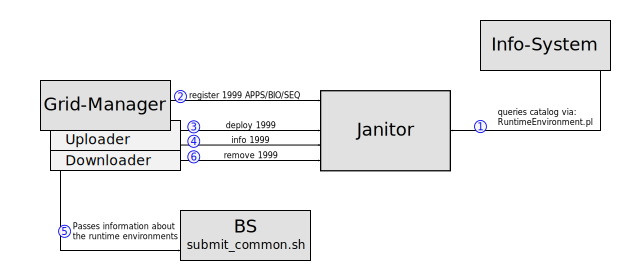
\includegraphics[width=12cm]{images/janitor_integration_2nd_edition.pdf}
    \mycaption{}{}
    \label{fig:RE_states}
  \end{center}
\end{figure}

\section{WebService Interface}

Default port number: 55555\\
Client command equal, except assignment of HED.xml\\
 (from /arc1/trunk:12561)

\begin{figure}[!h]
  \begin{center}
    \includegraphics[width=12cm]{images/WS_structure.pdf}
    \mycaption{}{\task{To be translated and beautificated. SVG file is missing!}}
    \label{fig:RE_states}
  \end{center}
\end{figure}

Proposal for SOAP messages:\\
 namespace: dynamicruntime or janitor\\
\task{Create WSDL files for that}
\task{Permission concepts: Depending on certificates. Certain certificates may \texttt{sweep}. Defined in service\_HED.xml. Evaluated in:?? }
\lstsetJUSTXML
\begin{lstlisting}[
        label=lst:SOAPrequest,
        caption={ [Example \textit{arc.conf} settings for janitor.]
                  \textbf{Example \textit{arc.conf} settings for janitor.}}
        ]
<Request action="SEARCH|SWEEP|LIST|DEPLOY|REMOVE|CHECK|REGISTER">
	<Initiator jobid="1234"/>  <!-- Needed for: CHECK|REGISTER|DEPLOY|REMOVE -->
                                  <!-- May contain no jobID in this case a new one will 
                                       be created and returned via the response message-->

	<Runtimeenvironment type="dynamic">      <!-- Needed for: SEARCH|REGISTER-->
		<Package name="APPS/BIO/WEKA-3.4.10"/>
		<Package name="APPS/BIO/WEKA-3.4.11"/>
	</Runtimeenvironment>
                                  <!-- SWEEP and LIST only works, if the TLS-adminstrator identity 
                                       (which is assigned in the arched configuration file) is
                                       to be found by the SecHandler. Both need neither initiator 
                                       nor runtimeenvironment elements -->
</Request>
\end{lstlisting}

\lstsetJUSTXML
\begin{lstlisting}[
        label=lst:SOAPrequest,
        caption={ [Example \textit{arc.conf} settings for janitor.]
                  \textbf{Example \textit{arc.conf} settings for janitor.}}
        ]
<response action="SEARCH|SWEEP|LIST|DEPLOY|REMOVE|CHECK|REGISTER">
	<initiator jobid="1234"/>  <!-- Needed for REMOVE|REGISTER|DEPLOY|CHECK-->
	<result code="0" message="Sucessfully initailized job."> <!-- -->
	<jobs> <!--LIST|CHECK-->
		<job jobid="1234">
			<created>1234567890</created>    <!-- in unix time-->
			<age>0</age>           <!-- in seconds-->
			<runtimeenvironment>
				<package>APPS/BIO/WEKA-3.4.10</package>
			</runtimeenvironment>
			<state>INITIALIZED</state>
		</job>
		<job jobid="4321">
			<created>1234567891</created>
			<age>0</age>
			<package>APPS/BIO/WEKA-3.4.10</package>
			<state>INITIALIZED</state>
			<runtimeenvironmentkey>APPS_BIO_WEKA_3_4_10-835614b62c98c4eb6cb03d74d3161b5d</runtimeenvironmentkey> <!-- at least CHECK -->
			<uses>/nfshome/knowarc/dredesign/src/services/dRE3/perl/spool/runtime/jre__57T1ke1UVz/runtime</uses> <!-- at least CHECK -->
			<uses>/nfshome/knowarc/dredesign/src/services/dRE3/perl/spool/runtime/weka_wHfyytarlE/runtime</uses> <!-- at least CHECK -->
		</job>
	</jobs>

	<runtimeenvironment type="local">      <!-- Needed for: LIST|SEARCH -->
		<package name="APPS/BIO/MUSTANG-3.0-1"/>
		<package name="APPS/BIO/EXONERATE-2.1.0-1"/>
	</runtimeenvironment>

	<runtimeenvironment type="dynamic">      <!-- Needed for: LIST -->
		<package name="APPS/BIO/WEKA-3.4.11">
			<state>INSTALLED_A</state>
			<lastused>1234567890</lastused>
			<jobid>1234</jobid>
		</package>
		<package name="APPS/BIO/WEKA-3.4.10">
			<state>INSTALLED_A</state>
			<lastused>1234567890</lastused>
			<jobid>1234</jobid>
			<jobid>4321</jobid>
		</package>
	</runtimeenvironment>

	<runtimeenvironment type="installable">      <!-- Needed for: LIST -->
		<package name="APPS/GRAPH/POVRAY-3.6">
			<description>The Persistence of Vision Raytracer</description>
			<lastupdate>1234567890</lastupdate>
		</package>
		<package name="APPS/BIO/WEKA-3.4.8A">
			<description>WEKA Machine Learning Software</description>
			<lastupdate>1234567890</lastupdate>
		</package>
	</runtimeenvironment>

</response>
\end{lstlisting}




\section{Janitor file system permissions}

In the current implementation the Janitor perl scripts must be executed as root. In order to execute Janitor with the required permissions,
a setuid wrapper has been prepared. During the installation \task{not done yet} the mode of rjanitor will be set to \texttt{u+s},
i.e. the sticky bit is set to make the binary suid root. \task{According to Daniel: ``A future version of the Janitor will get rid of the suid root helper.''}\\

Thus, Janitor is not executed directly. Instead, a dynamic link will be created in \task{libexec or sbin} which is pointing to
the wrapper.\\

It is suggested to create a user and a group "janitor" for the Janitor.\\

% Currently the Janitor must be executed as root. For this a suid root helper
% is needed. It is provided in /opt/janitor/rjanitor.c. If you installed
% the Janitor in another directory then /opt/janitor change the parameter
% of the execv command in rjanitor.c. Then compile the file with\\
% \texttt{\textdollar gcc -o rjanitor rjanitor.c}\\
% and run as root\\
% \texttt{\textdollar chown root:root rjanitor}\\
% \texttt{\textdollar chmod u+s rjanitor}\\
% to make the binary suid root. A future version of the Janitor will get rid
% of the suid root helper.\\
% 
% The Grid Manager does not call the Janitor directly in /opt/janitor but
% calls /opt/nordugrid/libexec/janitor. So a link is needed (as root):\\
% \texttt{\textdollar ln -s /opt/janitor/rjanitor /opt/nordugrid/libexec/janitor}\\
% \\
% It is suggested to create a user and a group "janitor" for the Janitor.\\
% \\
% The Janitor needs a directory for storing information on installed REs:\\
% \texttt{\textdollar mkdir -p /var/lib/nordugrid/janitor}\\
% \texttt{\textdollar chown janitor:janitor /var/lib/nordugrid/janitor}\\
% \\
% It also needs a directory on the shared volume for installing the REs:\\
% % \texttt{\textdollar mkdir -p $<$shared_volume$>$/janitor}\\
% % \texttt{\textdollar chown janitor:janitor $<$shared_volume$>$/janitor}


\subsection{What happens during installation}

Register
\begin{enumerate}
 \item Look up Catalog and find corresponding runtime environments.
 \item Check if dependcies are available (installed or installable)
 \item Store job in \textit{registrationdir}
\end{enumerate}

Deploy
\begin{enumerate}
 \item Load job out of \textit{registrationdir}
 \item Look up Catalog and find corresponding runtime environments.
 \item Check if dependcies are available (installed or installable)
 \item Download RTEs into the \textit{downloaddir}
 \item $\lbrack$ to be continued or skipped $\rbrack$
\end{enumerate}

\subsection{Security Consideration}



Security is a major concern for grid systems. Any additional feature
and especially an automatic software
installation inheritently introduces security threats. This section
addresses those and describes the available solutions to limit
security risks.

In the current installation, every user authorised to execute a job is
also authorised to install a REs. Restrictions are
only imposed on the set of dynamic REs that are available for installation.
Restrictions are imposed by the site admininistrators on the descriptions
that are given by the Catalog that is offering the package. These
descriptions may explicitly mention dynamic REs' names, e.g. a regular expression on
these, or refer to tags of packages that categorise these. However,
the core of these controls lies with the maintainers of the Catalog,
who needs to be trusted.

All dynamic REs are installed in separate directories. The provisioning of
disk space is the duty of the site administrator.  In the current
implementation, the installation is completely transparent to the user:

\begin{itemize}
\item Dynamic REs are not distinguished between {\em installed} and
  {\em installable} in the information system.
\item No status information is given at the time a dynamic RE is installed.
\end{itemize}

Malevolent regular users with respective training in using system exploits
to gain root access are likely to find security holes by regularly
submitted scripts.  The authentication and authentification of users,
together with respective logging, is the major defense against such
attacks. What is consequently left to be protected against are unwanted
side-effects by the installation of software.

The worst case scenario would be the installation of a RE
that overwrites system files. With the current implementation, which is
based solely on tar files, this is barely possible, unless such is
performed by the install scripts that accompany the tar files. However,
hereto the installation would have to be performed by a user with system
priviledges, for which there is no technical requirement.

The installation of packages from the Debian distribution (or other
packages of mainstream Linux distributions) is seeked to reduce the
complexity and burden in the maintenance for dynamic REs. In the
current implementation, Debian packages may be installed only by their
transformation into tar files. With the advent of the interface for
the virtualisation of the grid infrastructure, it is anticipated to
work with native packages of the Debian Linux distribution. The reuse
of packages that passed many eyeballs - as it is the case with packages
from major Linux distribution - security is further increased or becomes
as high as with the operating system underneath virtual clients.

Summarising, there is general concern about the security of grid
computing.  Dynamic REs introduce new dangers since a
manual control at the grid site is substituted by a remote process that
is out the direct supervision of a local site administrator. The signing
of packages by known and directly or indirectly trusted developers is
a good indicator that no malevolent individuals have tampered with the
binary. The site administrators can limit the sources of packages and
specify packages that are eligible or excluded from installations.



% * Programming concept
% ** design decisions: Perl, RDF, Two classes entities with states: jobs and rtes
% ** State transitions of RTEs
% ** State transitions of Jobs
% ** RDF based knowledge base for runtime environments
% ** File based recovery of Jobs and RTEs
% ** Class structure
% ** Interaction with A-REX
% 
